% introduction/set01-intro.tex — discrete probability foundations, Bernoulli, CLT teaser, Gaussian / empirical rule
% Included before Core Formulas in HSC-Distributions.tex

\subsection{Random experiments and random variables}

Throwing four fair coins and recording the number of heads is a \textbf{random experiment} because more than one outcome is possible. Throwing four coins into an empty bucket and counting how many coins are in the bucket is a \textbf{deterministic experiment} because the outcome is necessarily~4.

A \textbf{(discrete) random variable} attaches a numerical value to each outcome of such an experiment.

\subsection{Discrete probability distributions}

Suppose the sample space of an experiment can be listed (written down in order) and the possible outcomes are numeric. Those outcomes together with their probabilities form a \textbf{discrete probability distribution}.

\textbf{Probability mass function (PMF).} If $X$ takes values $x_1,x_2,\ldots$ then the PMF is $p(x)=P(X=x)$ where $p(x_i)\geq 0$ and $\sum_i p(x_i)=1$.
For example, let $X$ be the number of heads in three fair tosses of a coin. Then $X\in\{0,1,2,3\}$ with
\begin{align*}
P(X=0) &= \tfrac{1}{8}, &
P(X=1) &= \tfrac{3}{8}, &
P(X=2) &= \tfrac{3}{8}, &
P(X=3) &= \tfrac{1}{8}.
\end{align*}
Each probability is computed by counting equiprobable sequences (e.g.\ $P(X=2)=\binom{3}{2}(\tfrac12)^3$).

\subsection{Uniform discrete distributions}

A discrete distribution is \textbf{uniform} when every outcome in its sample space has the same probability --- the values are equally likely. For instance, rolling a fair six-sided die and recording the upper face produces a uniform distribution on $\{1,2,3,4,5,6\}$ with $P(X=k)=\tfrac16$ for each~$k$.

\subsection{Bernoulli trials and binomial experiments}

A \textbf{Bernoulli trial} is a single random experiment with exactly two outcomes, often called ``success'' and ``failure'', with probabilities $p$ and $q=1-p$. Tossing a coin once with success $=$ heads gives $p=\tfrac12$. Throwing a die once and recording only whether a six appears is a Bernoulli trial with $p=\tfrac16$ if success is ``six''.

A \textbf{binomial experiment} consists of $n$ independent Bernoulli trials, each with the same success probability~$p$, and the random variable $X$ is the total number of successes (order of successes does not matter). For example, tossing the same coin five times and counting heads is a binomial experiment with $n=5$. If each toss is independent with probability~$p$ of heads,
\[
P(X=k)=\binom{n}{k} p^k(1-p)^{n-k},\qquad k=0,1,\ldots,n.
\]
The table below lists outcomes for five fair tosses ($p=\tfrac12$):

\begin{center}
\begin{tabular}{|c|c|c|c|c|c|c|}
\hline
$k$ (heads) & 0 & 1 & 2 & 3 & 4 & 5 \\
\hline
$P(X=k)$ & $\frac{1}{32}$ & $\frac{5}{32}$ & $\frac{10}{32}$ & $\frac{10}{32}$ & $\frac{5}{32}$ & $\frac{1}{32}$ \\
\hline
\end{tabular}
\end{center}

\subsection{Improper integrals}

For continuous models, probabilities often use integrals on unbounded intervals, for example
\[
P(X\le a)=\int_{-\infty}^{a} f(x)\,dx,\qquad
P(X\in\mathbb{R})=\int_{-\infty}^{\infty} f(x)\,dx.
\]
Such \textbf{improper integrals} are evaluated as limits of proper integrals (e.g.\ $\int_{-\infty}^{\infty}=\lim_{b\to\infty}\int_{-b}^{b}$ when the limit exists). Checking that $\int_{-\infty}^{\infty} f(x)\,dx=1$ confirms that $f$ can be a valid pdf.

\subsection{A first look at the Central Limit Theorem}

Let independent observations $X_1,\ldots,X_n$ share mean $\mu$ and variance $\sigma^2$, and define the sample mean $\overline{X}=\frac1n\sum_{i=1}^n X_i$. Under mild conditions, for large $n$ the distribution of $\overline{X}$ is approximately normal with
\[
E(\overline{X})=\mu,\qquad \mathrm{Var}(\overline{X})=\frac{\sigma^2}{n},\qquad \mathrm{s.d.}(\overline{X})=\frac{\sigma}{\sqrt{n}}.
\]
\textbf{Central limit idea:} the distribution of means of many independent draws becomes approximately normal even when the original variable is not. That is why the normal distribution appears throughout statistics, for both discrete and continuous models.

\subsection{Gaussian (normal) distributions and the empirical rule}

The \textbf{normal} (Gaussian) family includes the standard normal $Z\sim N(0,1)$ and $X\sim N(\mu,\sigma^2)$ with pdf the familiar bell curve. The mean locates the centre; the standard deviation~$\sigma$ measures spread.

\textbf{Empirical rule (68--95--99.7).} For a normal distribution, approximately
\begin{itemize}[leftmargin=*]
  \item 68\% of values lie within one standard deviation of the mean ($\mu\pm\sigma$);
  \item 95\% within two standard deviations ($\mu\pm 2\sigma$);
  \item 99.7\% within three standard deviations ($\mu\pm 3\sigma$).
\end{itemize}

\begin{center}
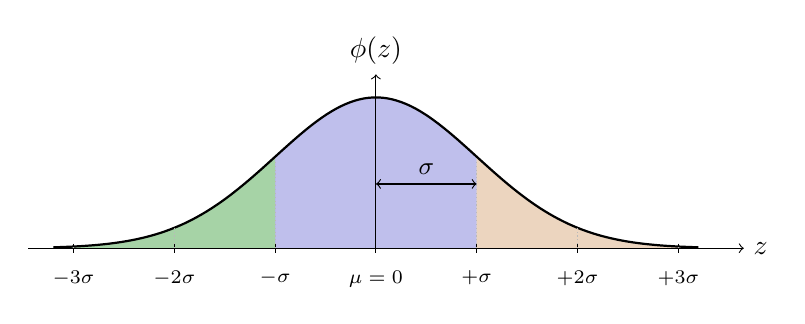
\begin{tikzpicture}[
    x=1.28cm,
    y=4.8cm,
    declare function={ gauss(\x) = exp(-0.5*(\x)^2)/(sqrt(2*pi)); }
]
\begin{scope}
  \fill[green!50!black, opacity=0.35]
    (-3.2,0) -- plot[domain=-3.2:-1.0, samples=40] (\x,{gauss(\x)}) -- (-1.0,0) -- cycle;
  \fill[blue!70!black, opacity=0.25]
    (-1.0,0) -- plot[domain=-1.0:1.0, samples=40] (\x,{gauss(\x)}) -- (1.0,0) -- cycle;
  \fill[orange!70!black, opacity=0.25]
    (1.0,0) -- plot[domain=1.0:3.2, samples=40] (\x,{gauss(\x)}) -- (3.2,0) -- cycle;
  \draw[->] (-3.45,0) -- (3.65,0) node[right] {$z$};
  \draw[->] (0,0) -- (0,0.46) node[above] {$\phi(z)$};
  \draw[thick, domain=-3.2:3.2, samples=140] plot (\x,{gauss(\x)});

  \foreach \x/\lab in {
    -3/{$-3\sigma$},
    -2/{$-2\sigma$},
    -1/{$-\sigma$},
     0/{$\mu=0$},
     1/{$+\sigma$},
     2/{$+2\sigma$},
     3/{$+3\sigma$}
  }{
    \draw (\x,0.012) -- (\x,-0.012)
      node[below=3pt, font=\scriptsize] {\lab};
  }

  \foreach \x in {-3,-2,-1,1,2,3}{
    \draw[densely dotted, gray!55] (\x,0) -- (\x,{gauss(\x)});
  }
  \draw[<->] (0,0.17) -- (1,0.17)
    node[midway, above, font=\small] {$\sigma$};
\end{scope}
\end{tikzpicture}
\end{center}
\noindent\textit{Figure: standard normal curve $z\mapsto \phi(z)$ with mean at $0$, standard-deviation markers on the $z$-axis, and shaded bands illustrating central and tail regions.}
